The implementation of the small-signal stability analysis is divided mainly into two parts: the code development
 and the GUI implementation. 

\subsubsection{Code development}

The small-signal stability analysis is implemented in Python, following the general structure of the 
dynamic simulation framework in Veragrid. The general simulation structure for any simulation in VeraGrid
 is shown in Figure \ref{fig:General_Simulation_Structure}. 

\begin{figure}[H]
  \centering
  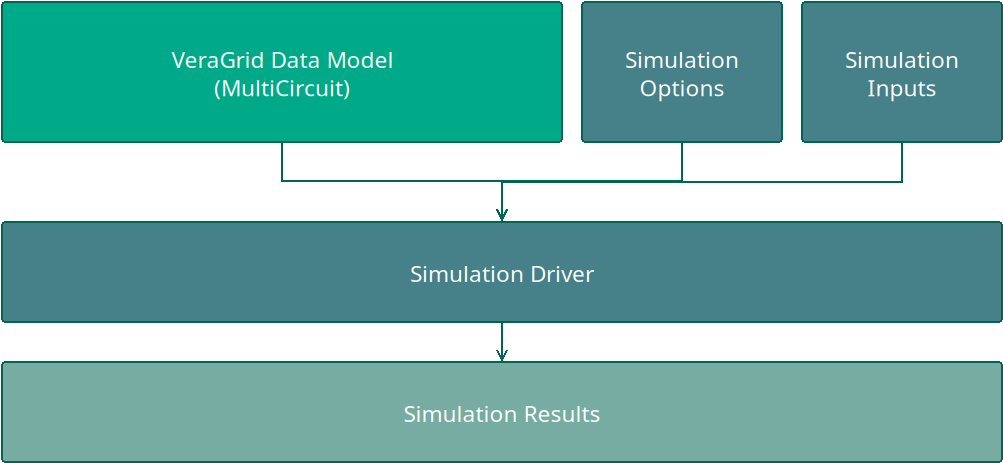
\includegraphics[width=0.8\linewidth]{figures/DataModelSimulationStructure.png}
  \caption{General simulation structure. \textit{Source: VeraGrid documentation \cite{veragrid}}}
  \label{fig:General_Simulation_Structure}
\end{figure}

Therefore, each simulation has three main classes explained below:

\begin{itemize}
    \item \textbf{Driver:} This class is responsible for running the simulation. It contains the simulation analysis function itself
    that computes the results and the run function that is called from the GUI, and it is responsible for executing the simulation.

    The block diagram of the small-signal stability analysis simulation function is shown in Figure \ref{fig:block_diagram_run_smallsignal}. 
    It consists on the A matrix computation from the jacobian matrix, the eigenvalues computation and then 2 main postprocesses: the participation factors
    computation and the damping ratios and oscillation frequencies computation. 
    
    The full simulation block diagram is shown in Figure \ref{fig:block_diagram_full_smallsignal} where one can see the main steps of the simulation from 
    importing the system data to the final results. The approach given is to give the user the option to run the small-signal stability analysis
    whenever he/she wants in the dynamic simulation. The user can initialize the system, check the stability in the first operation point, add an event and
    then check the stability again in the new operation point just choosing the assessment time.

    \item \textbf{Results:} This class is responsible for storing the results of the simulation. It contains the data structure that holds the results
    and the way they are accessed from the GUI. In this case, the results class show three main results: the eigenvalues with their corresponding damping ratios
    and oscillation frequencies, the participation factors matrix with the corresponding eigenvalues and states for each column and row respectively,
    and the complex plane plot of the eigenvalues in bot $rad/s$ and $Hz$ for the imaginary axis.

    \item \textbf{Options:} This class is responsible for defining the options of the simulation. It contains the parameters that can be set by the user
    from the GUI. In this case, the options class allows the user to set the assessment time, and in case the dynamic simulation is needed,
     the options for the simulation: integration method, time step and tolerance.
    
\end{itemize}

\begin{figure}[h]
  \centering
  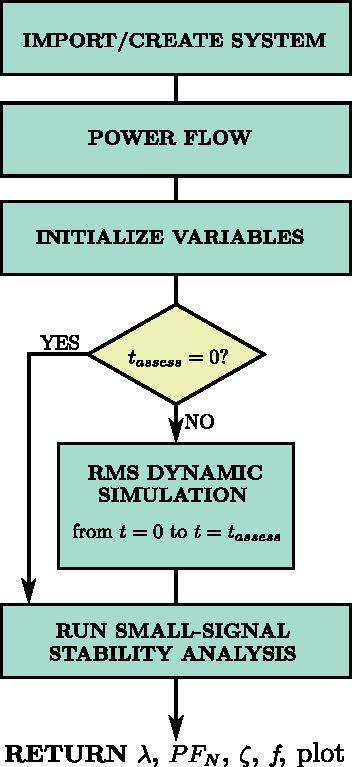
\includegraphics[width=0.35\linewidth]{inkscape_svg/block_diagram_full_code_smallsignal.pdf}
  \caption{Small-signal stability analysis full simulation block diagram. \textit{Source: Own elaboration.}}
  \label{fig:block_diagram_full_smallsignal}
\end{figure}

\begin{figure}[H]
  \centering
  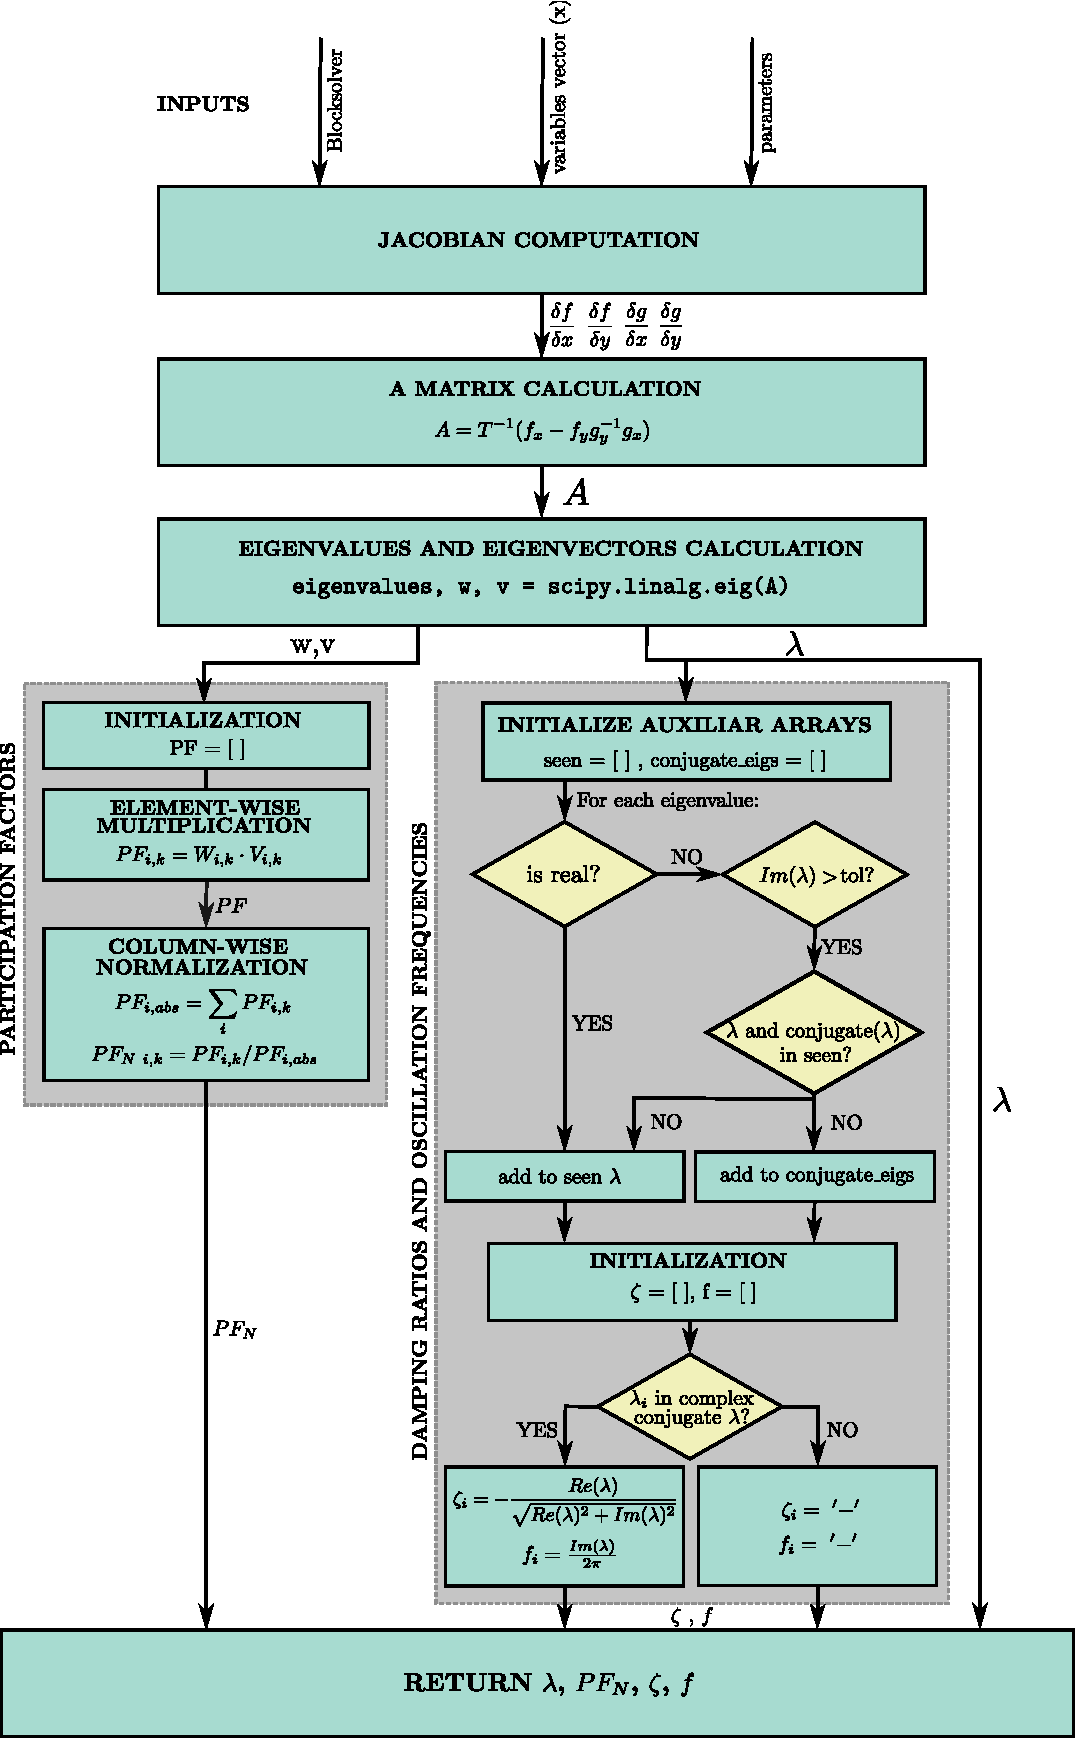
\includegraphics[width=0.8\linewidth]{inkscape_svg/block_diagram_run_smallsignal.pdf}
  \caption{Small-signal stability analysis computation block diagram. \textit{Source: Own elaboration.}}
  \label{fig:block_diagram_run_smallsignal}
\end{figure}

\subsubsection{GUI implementation}

The GUI is creased using the open source program Qt Designer \cite{qt_designer}, which allows to create the GUI using a drag 
and drop interface. The GUI implementation consists on creating a new settings page for the small-signal stability analysis,
adding the option to run the simulation in the main tools bar, and creating a new results page to show the results of the simulation. 
The GUI implementationis not only adding the new pages, but also connecting the GUI with the code developed in Python.

However, the first initial step is to choose an icon for the small-signal stability analysis that will be shown in the tools bar and will 
hels users identify the option. The icon chosen is shown in Figure \ref{fig:small_signal_icon}. The icon represents a magnifying glass 
looking at a wave. The magnifying glass represents the small-signal analysis, which works around a small perturbation and a small interval
around the operating point, so the user needs the magnifying glass to see those small perturbations. The wave represents the system variables
represented in the time domain, which are the ones that will be analysed in the small-signal stability analysis.

\begin{figure}[H]
  \centering
  
\includegraphics[width=0.25\linewidth]{inkscape_svg/small_signal_icon.pdf}
  \caption{Icon for the small-signal stability analysis. \textit{Source: VeraGrid \cite{veragrid}.}}
  \label{fig:small_signal_icon}
\end{figure}

The settings page shown in Figure \ref{fig:smallsignal_settings_GUI} allows the user to set the parameters needed for the small-signal stability analysis.
It is noted how the small-signal settings are added into the dynamic simulation settings. The settings shown are explained in the list below.

\begin{enumerate}
  \item \textit{Integration method}: The integration method to use if the RMS dynamic simulation is performed. There are two options: trapezoidal or implicit euler.
  \item \textit{Tolerance}: per-unit error tolerance to use in the integration method. Only needed if the Rms dynamic simulation is performed.
  \item \textit{Assessment time (s)}: The time instant in seconds where the stability assessment is performed.
  \item \textit{Time step (s)}: Step size in seconds between each numerical evaluation in the integration method. 
  Smaller intervals increase accuracy but require more computation. Only needed if the RMS dynamic simulation is performed.
\end{enumerate}


\begin{figure}[H]
  \centering
  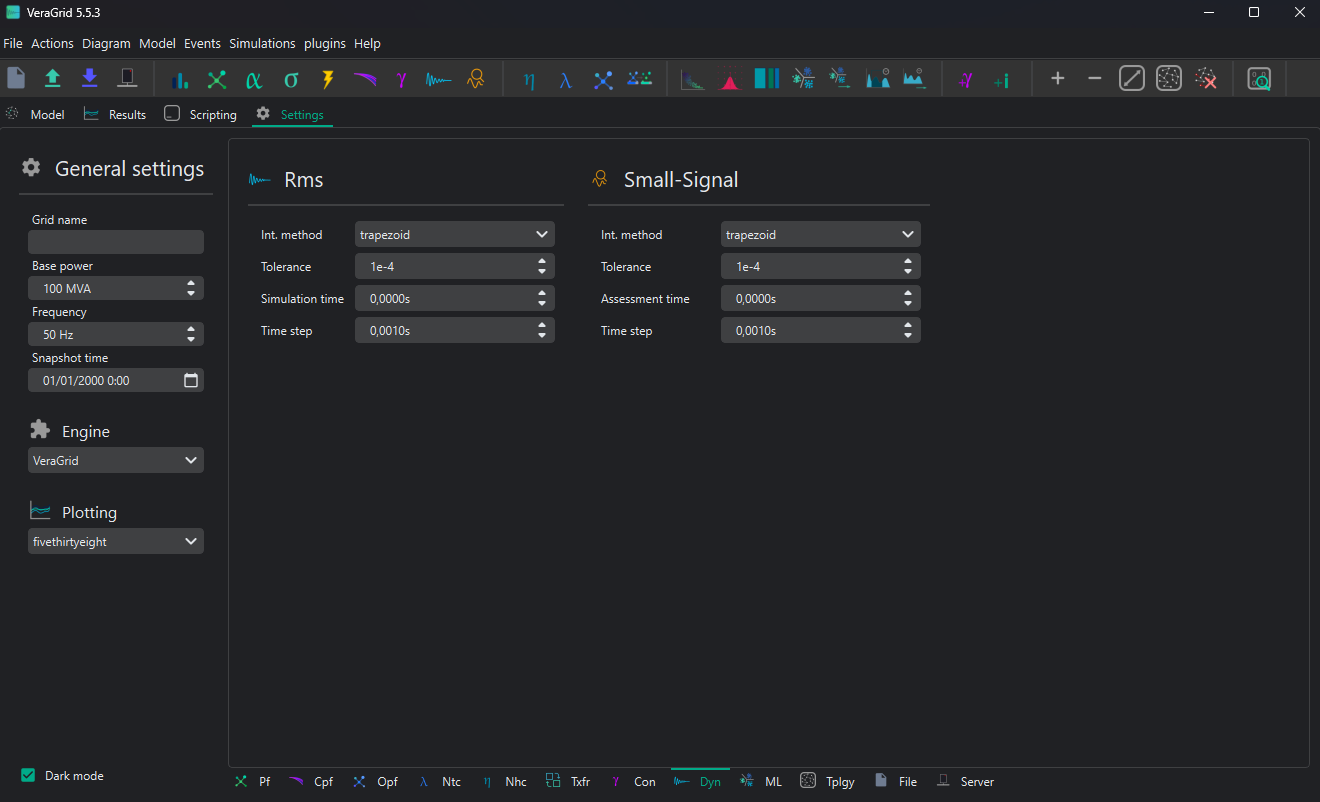
\includegraphics[width=0.8\linewidth]{figures/settings_GUI.png}
  \caption{Small-signal stability analysis settings page. \textit{Source: VeraGrid \cite{veragrid}.}}
  \label{fig:smallsignal_settings_GUI}
\end{figure}

Figure \ref{fig:model_powerflow_GUI} shows the model page with the power flow already computed. The small-signal stability analysis can 
only be performed if the power flow has been computed, as it is needed to obtain the operating point of the system.

\begin{figure}[H]
  \centering
  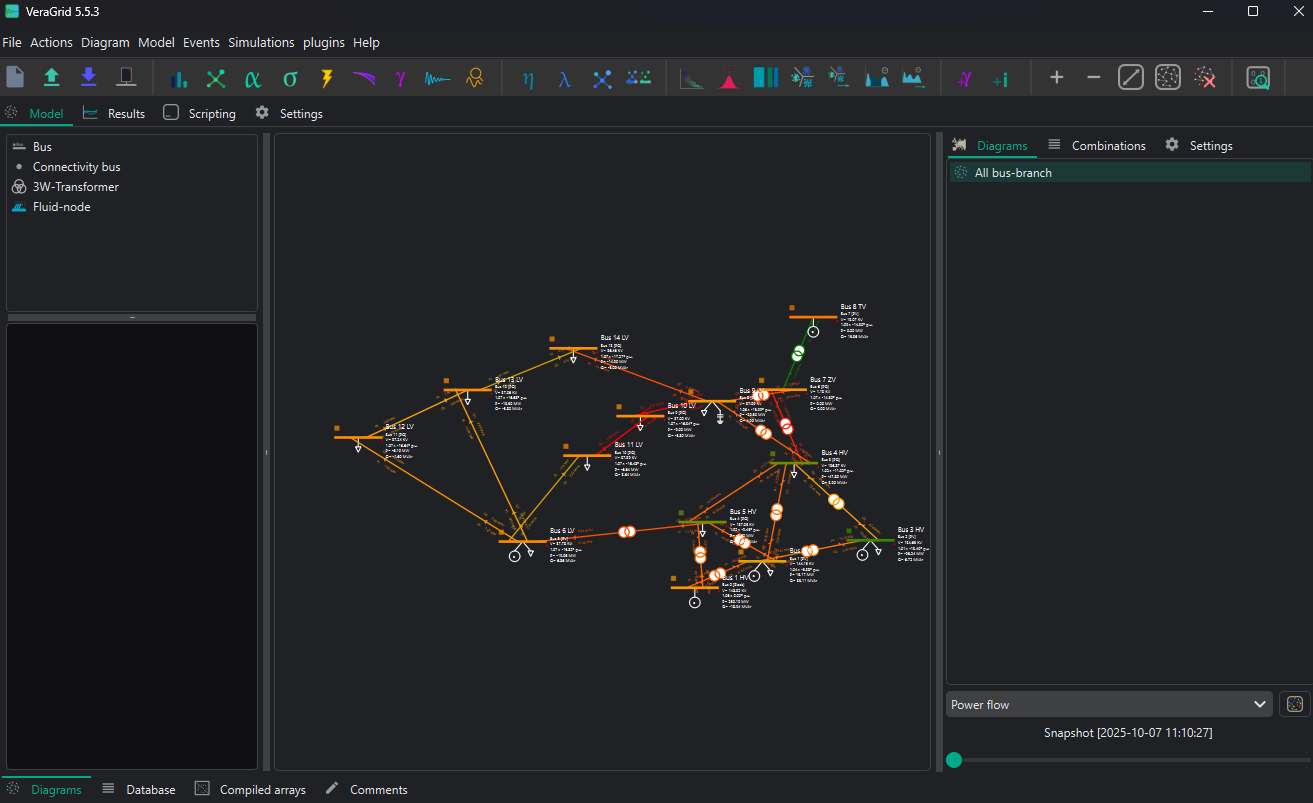
\includegraphics[width=0.8\linewidth]{figures/model_powerflow_GUI.png}
  \caption{Model page with power flow already computed. \textit{Source: VeraGrid \cite{veragrid}.}}
  \label{fig:model_powerflow_GUI}
\end{figure}

\begin{figure}[H]
  \centering
  \begin{minipage}{0.45\textwidth}
    \centering
    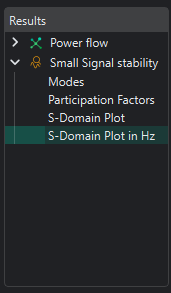
\includegraphics[width=0.5\linewidth]{figures/results_desplegable_GUI.png}
    \caption{Results drowdown. \textit{Source: VeraGrid \cite{veragrid}.}}
    \label{fig:results_dropdown_GUI}
  \end{minipage}
  \hfill
  \begin{minipage}{0.5\textwidth}
    The results page shows the results of all the simulations performed in VeraGrid. The user can choose the results to show
    using the dropdown menu shown in Figure \ref{fig:results_dropdown_GUI}. In this case, the power flow and small-signal stability
     analysis results are shown. As one can see, the small-signal results are divided into 4 options: the modes table, the participation
     factors table, the complex domain plot and the complex domain plot in Hz. These results are shown in Figures \ref{fig:table_modes_GUI},
     \ref{fig:table_PF_GUI}, \ref{fig:plot_ss_GUI} and \ref{fig:plot_ss_Hz_GUI} respectively.
  \end{minipage}
\end{figure}

\begin{figure}[H]
  \centering
  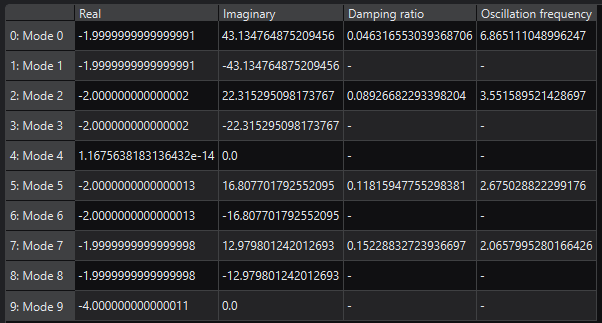
\includegraphics[width=0.8\linewidth]{figures/result_modes_ss_GUI.png}
  \caption{Table result with the modes, damping ratio and oscillation frequencies. \textit{Source: VeraGrid \cite{veragrid}.}}
  \label{fig:table_modes_GUI}
\end{figure}

\begin{figure}[H]
  \centering
  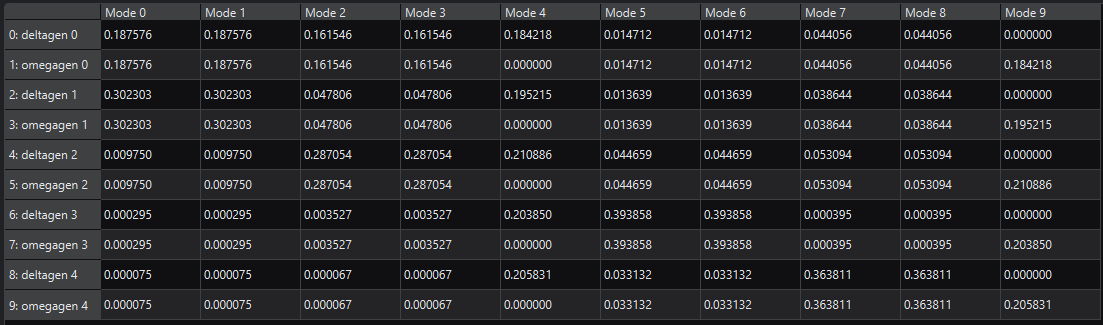
\includegraphics[width=1\linewidth]{figures/result_pfactors_GUI.png}
  \caption{Table result with the participation factors. \textit{Source: VeraGrid \cite{veragrid}.}}
  \label{fig:table_PF_GUI}
\end{figure}

\begin{figure}[H]
  \centering
  \begin{minipage}{0.49\textwidth}
    \centering
    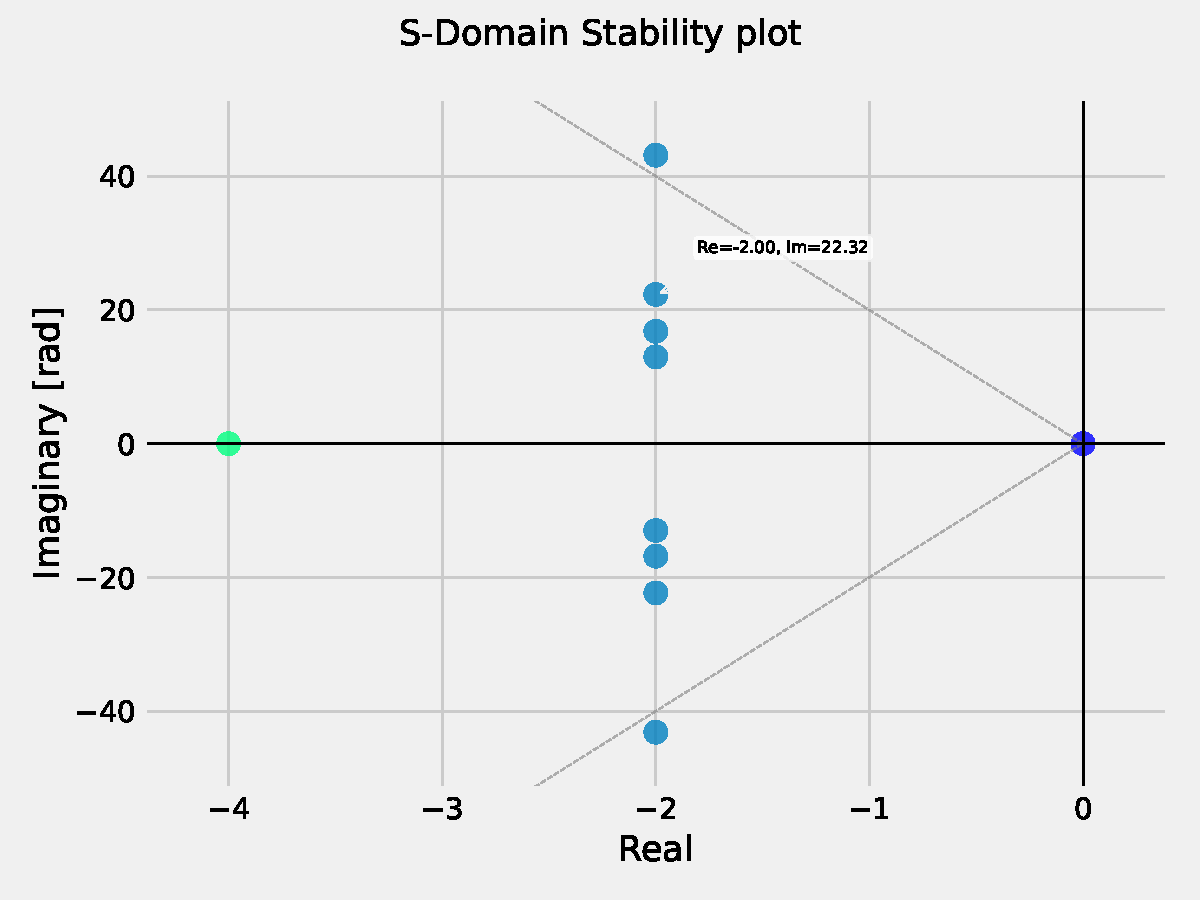
\includegraphics[width=\linewidth]{figures/smallsignal_plot_GUI.pdf}
    \caption{Complex domain plot.  \textit{Source: VeraGrid \cite{veragrid}.}}
    \label{fig:plot_ss_GUI}
  \end{minipage}
  \hfill
  \begin{minipage}{0.49\textwidth}
    \centering
    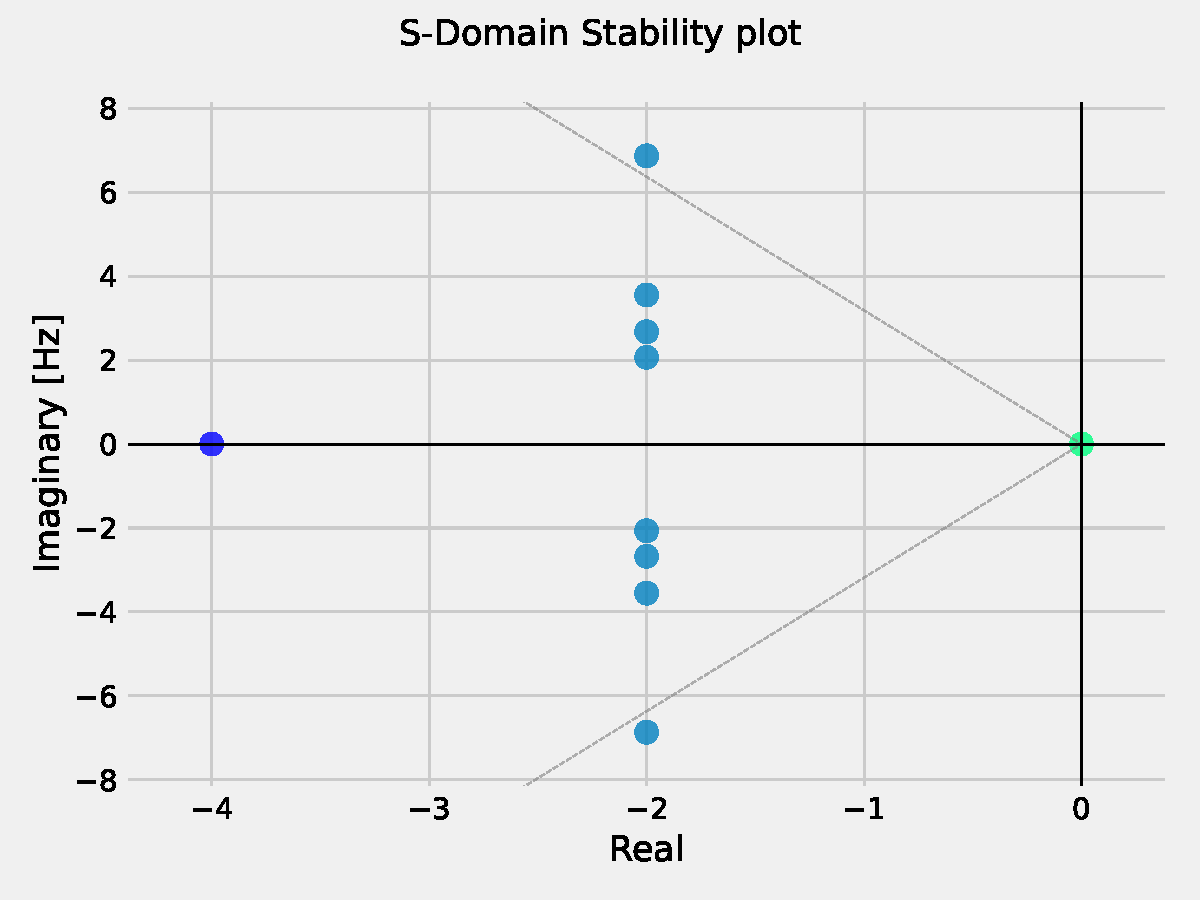
\includegraphics[width=\linewidth]{figures/smallsignal_plot_Hz_GUI.pdf}
    \caption{Complex domain plot in Hz. \textit{Source: VeraGrid \cite{veragrid}.}}
    \label{fig:plot_ss_Hz_GUI}
  \end{minipage}
\end{figure}

Figure \ref{fig:plot_ss_GUI} shows how the user can take a look at the eigenvalues exact values
by hovering the mouse over the points. Moreover, the 5\% damping ratio line is shown to help the user identify
the unstable modes. 








